
%(BEGIN_QUESTION)
% Copyright 2010, Tony R. Kuphaldt, released under the Creative Commons Attribution License (v 1.0)
% This means you may do almost anything with this work of mine, so long as you give me proper credit

Calculate the appropriate millivoltage values and potentiometer resistances to simulate a thermocouple at the desired temperatures, assuming the ambient temperature at the transmitter is 72 $^{o}$F and the transmitter has cold junction compensation {\it enabled}:

$$\includegraphics[width=15.5cm]{i03657x01.eps}$$

\begin{itemize}
\item{} $T_{simulate}$ = 550 $^{o}$F ; $V_{input}$ = \underbar{\hskip 50pt} mV ; $R_{pot}$ = \underbar{\hskip 50pt} $\Omega$
\vskip 10pt
\item{} $T_{simulate}$ = 300 $^{o}$F ; $V_{input}$ = \underbar{\hskip 50pt} mV ; $R_{pot}$ = \underbar{\hskip 50pt} $\Omega$
\vskip 10pt
\item{} $T_{simulate}$ = 150 $^{o}$F ; $V_{input}$ = \underbar{\hskip 50pt} mV ; $R_{pot}$ = \underbar{\hskip 50pt} $\Omega$
\end{itemize}

\underbar{file i03657}
%(END_QUESTION)





%(BEGIN_ANSWER)

\begin{itemize}
\item{} $T_{simulate}$ = 550 $^{o}$F ; $V_{input}$ = {\bf 14.516} mV ; $R_{pot}$ = {\bf 741.39} $\Omega$
\vskip 10pt
\item{} $T_{simulate}$ = 300 $^{o}$F ; $V_{input}$ = {\bf 6.815} mV ; $R_{pot}$ = {\bf 347.80} $\Omega$
\vskip 10pt
\item{} $T_{simulate}$ = 150 $^{o}$F ; $V_{input}$ = {\bf 2.278} mV ; $R_{pot}$ = {\bf 116.20} $\Omega$
\end{itemize}

%(END_ANSWER)





%(BEGIN_NOTES)

%INDEX% Measurement, temperature: thermocouple millivoltage calibration

%(END_NOTES)

